% Created by tikzDevice version 0.10.1 on 2020-02-15 16:08:50
% !TEX encoding = UTF-8 Unicode
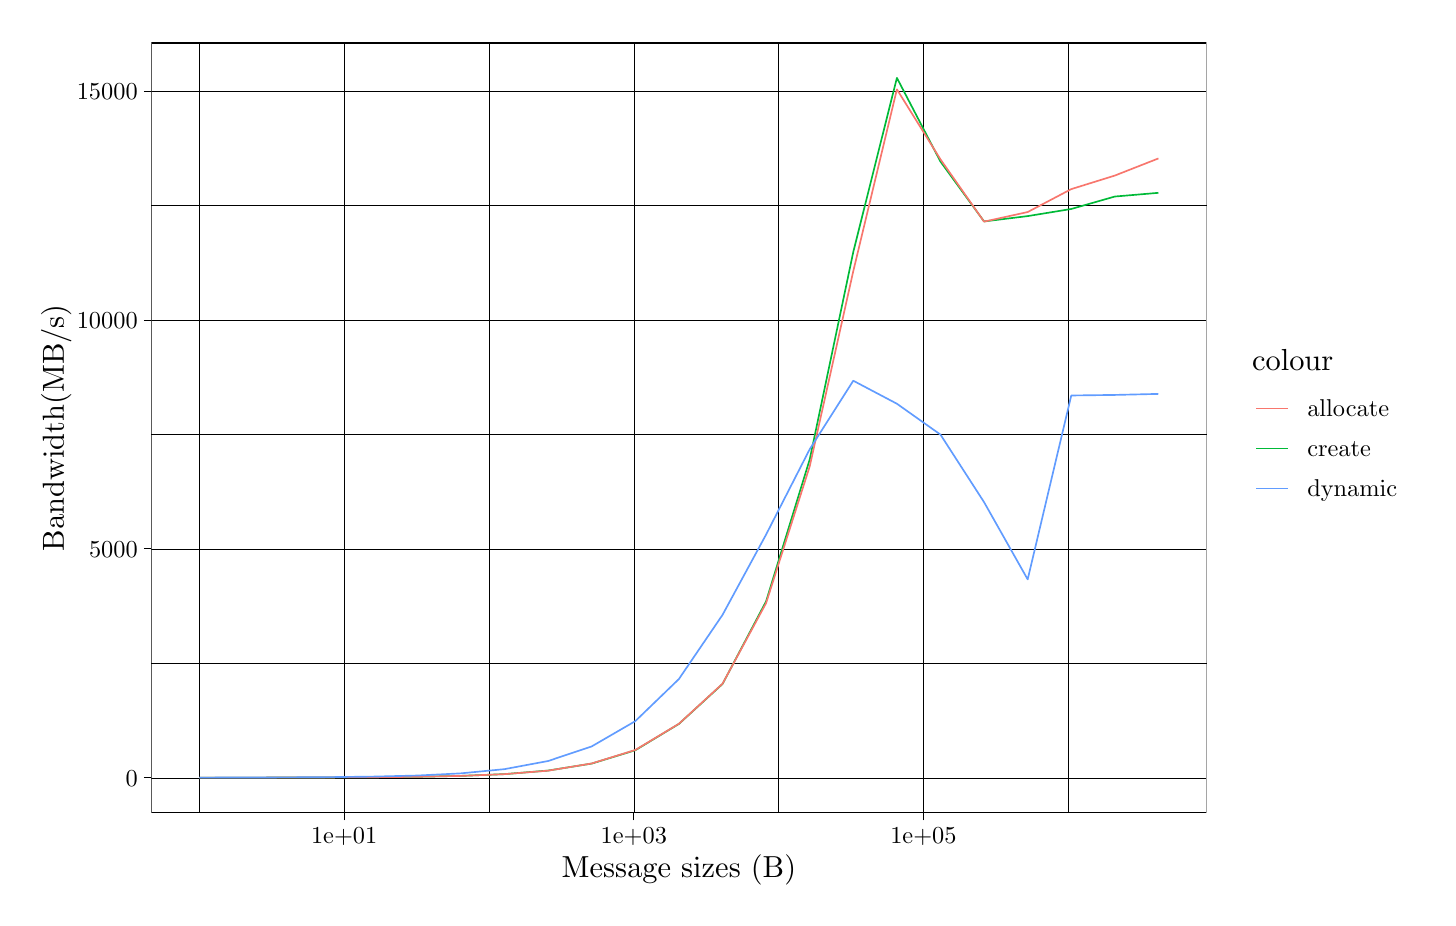
\begin{tikzpicture}[x=1pt,y=1pt]
\definecolor{fillColor}{RGB}{255,255,255}
\path[use as bounding box,fill=fillColor,fill opacity=0.00] (0,0) rectangle (505.89,314.37);
\begin{scope}
\path[clip] (  0.00,  0.00) rectangle (505.89,314.37);
\definecolor{drawColor}{RGB}{255,255,255}
\definecolor{fillColor}{RGB}{255,255,255}

\path[draw=drawColor,line width= 0.6pt,line join=round,line cap=round,fill=fillColor] (  0.00,  0.00) rectangle (505.89,314.37);
\end{scope}
\begin{scope}
\path[clip] ( 44.71, 30.72) rectangle (425.93,308.87);
\definecolor{fillColor}{RGB}{255,255,255}

\path[fill=fillColor] ( 44.71, 30.72) rectangle (425.93,308.87);
\definecolor{drawColor}{RGB}{0,0,0}

\path[draw=drawColor,line width= 0.0pt,line join=round] ( 44.71, 84.70) --
	(425.93, 84.70);

\path[draw=drawColor,line width= 0.0pt,line join=round] ( 44.71,167.39) --
	(425.93,167.39);

\path[draw=drawColor,line width= 0.0pt,line join=round] ( 44.71,250.08) --
	(425.93,250.08);

\path[draw=drawColor,line width= 0.0pt,line join=round] ( 62.04, 30.72) --
	( 62.04,308.87);

\path[draw=drawColor,line width= 0.0pt,line join=round] (166.70, 30.72) --
	(166.70,308.87);

\path[draw=drawColor,line width= 0.0pt,line join=round] (271.36, 30.72) --
	(271.36,308.87);

\path[draw=drawColor,line width= 0.0pt,line join=round] (376.02, 30.72) --
	(376.02,308.87);

\path[draw=drawColor,line width= 0.1pt,line join=round] ( 44.71, 43.36) --
	(425.93, 43.36);

\path[draw=drawColor,line width= 0.1pt,line join=round] ( 44.71,126.05) --
	(425.93,126.05);

\path[draw=drawColor,line width= 0.1pt,line join=round] ( 44.71,208.74) --
	(425.93,208.74);

\path[draw=drawColor,line width= 0.1pt,line join=round] ( 44.71,291.43) --
	(425.93,291.43);

\path[draw=drawColor,line width= 0.1pt,line join=round] (114.37, 30.72) --
	(114.37,308.87);

\path[draw=drawColor,line width= 0.1pt,line join=round] (219.03, 30.72) --
	(219.03,308.87);

\path[draw=drawColor,line width= 0.1pt,line join=round] (323.69, 30.72) --
	(323.69,308.87);
\definecolor{drawColor}{RGB}{0,186,56}

\path[draw=drawColor,line width= 0.6pt,line join=round] ( 62.04, 43.37) --
	( 77.80, 43.38) --
	( 93.55, 43.40) --
	(109.30, 43.44) --
	(125.05, 43.52) --
	(140.81, 43.68) --
	(156.56, 44.00) --
	(172.31, 44.64) --
	(188.07, 45.93) --
	(203.82, 48.45) --
	(219.57, 53.27) --
	(235.32, 62.78) --
	(251.08, 77.21) --
	(266.83,107.08) --
	(282.58,158.33) --
	(298.33,233.33) --
	(314.09,296.23) --
	(329.84,265.97) --
	(345.59,244.35) --
	(361.35,246.28) --
	(377.10,248.85) --
	(392.85,253.35) --
	(408.60,254.69);
\definecolor{drawColor}{RGB}{248,118,109}

\path[draw=drawColor,line width= 0.6pt,line join=round] ( 62.04, 43.37) --
	( 77.80, 43.38) --
	( 93.55, 43.40) --
	(109.30, 43.44) --
	(125.05, 43.52) --
	(140.81, 43.68) --
	(156.56, 44.00) --
	(172.31, 44.63) --
	(188.07, 45.89) --
	(203.82, 48.49) --
	(219.57, 53.37) --
	(235.32, 62.83) --
	(251.08, 77.30) --
	(266.83,106.45) --
	(282.58,155.83) --
	(298.33,226.39) --
	(314.09,292.08) --
	(329.84,266.78) --
	(345.59,244.28) --
	(361.35,247.75) --
	(377.10,256.03) --
	(392.85,260.93) --
	(408.60,267.12);
\definecolor{drawColor}{RGB}{97,156,255}

\path[draw=drawColor,line width= 0.6pt,line join=round] ( 62.04, 43.38) --
	( 77.80, 43.41) --
	( 93.55, 43.46) --
	(109.30, 43.55) --
	(125.05, 43.75) --
	(140.81, 44.13) --
	(156.56, 44.92) --
	(172.31, 46.44) --
	(188.07, 49.38) --
	(203.82, 54.66) --
	(219.57, 63.79) --
	(235.32, 79.00) --
	(251.08,102.18) --
	(266.83,131.21) --
	(282.58,162.03) --
	(298.33,186.79) --
	(314.09,178.48) --
	(329.84,167.32) --
	(345.59,142.91) --
	(361.35,115.01) --
	(377.10,181.46) --
	(392.85,181.66) --
	(408.60,182.03);
\definecolor{drawColor}{RGB}{0,0,0}

\path[draw=drawColor,line width= 0.6pt,line join=round,line cap=round] ( 44.71, 30.72) rectangle (425.93,308.87);
\end{scope}
\begin{scope}
\path[clip] (  0.00,  0.00) rectangle (505.89,314.37);
\definecolor{drawColor}{RGB}{0,0,0}

\node[text=drawColor,anchor=base east,inner sep=0pt, outer sep=0pt, scale=  0.88] at ( 39.76, 40.33) {0};

\node[text=drawColor,anchor=base east,inner sep=0pt, outer sep=0pt, scale=  0.88] at ( 39.76,123.02) {5000};

\node[text=drawColor,anchor=base east,inner sep=0pt, outer sep=0pt, scale=  0.88] at ( 39.76,205.71) {10000};

\node[text=drawColor,anchor=base east,inner sep=0pt, outer sep=0pt, scale=  0.88] at ( 39.76,288.40) {15000};
\end{scope}
\begin{scope}
\path[clip] (  0.00,  0.00) rectangle (505.89,314.37);
\definecolor{drawColor}{RGB}{0,0,0}

\path[draw=drawColor,line width= 0.3pt,line join=round] ( 41.96, 43.36) --
	( 44.71, 43.36);

\path[draw=drawColor,line width= 0.3pt,line join=round] ( 41.96,126.05) --
	( 44.71,126.05);

\path[draw=drawColor,line width= 0.3pt,line join=round] ( 41.96,208.74) --
	( 44.71,208.74);

\path[draw=drawColor,line width= 0.3pt,line join=round] ( 41.96,291.43) --
	( 44.71,291.43);
\end{scope}
\begin{scope}
\path[clip] (  0.00,  0.00) rectangle (505.89,314.37);
\definecolor{drawColor}{RGB}{0,0,0}

\path[draw=drawColor,line width= 0.3pt,line join=round] (114.37, 27.97) --
	(114.37, 30.72);

\path[draw=drawColor,line width= 0.3pt,line join=round] (219.03, 27.97) --
	(219.03, 30.72);

\path[draw=drawColor,line width= 0.3pt,line join=round] (323.69, 27.97) --
	(323.69, 30.72);
\end{scope}
\begin{scope}
\path[clip] (  0.00,  0.00) rectangle (505.89,314.37);
\definecolor{drawColor}{RGB}{0,0,0}

\node[text=drawColor,anchor=base,inner sep=0pt, outer sep=0pt, scale=  0.88] at (114.37, 19.71) {1e+01};

\node[text=drawColor,anchor=base,inner sep=0pt, outer sep=0pt, scale=  0.88] at (219.03, 19.71) {1e+03};

\node[text=drawColor,anchor=base,inner sep=0pt, outer sep=0pt, scale=  0.88] at (323.69, 19.71) {1e+05};
\end{scope}
\begin{scope}
\path[clip] (  0.00,  0.00) rectangle (505.89,314.37);
\definecolor{drawColor}{RGB}{0,0,0}

\node[text=drawColor,anchor=base,inner sep=0pt, outer sep=0pt, scale=  1.10] at (235.32,  7.44) {Message sizes (B)};
\end{scope}
\begin{scope}
\path[clip] (  0.00,  0.00) rectangle (505.89,314.37);
\definecolor{drawColor}{RGB}{0,0,0}

\node[text=drawColor,rotate= 90.00,anchor=base,inner sep=0pt, outer sep=0pt, scale=  1.10] at ( 13.08,169.80) {Bandwidth(MB/s)};
\end{scope}
\begin{scope}
\path[clip] (  0.00,  0.00) rectangle (505.89,314.37);
\definecolor{fillColor}{RGB}{255,255,255}

\path[fill=fillColor] (436.93,135.11) rectangle (500.39,204.49);
\end{scope}
\begin{scope}
\path[clip] (  0.00,  0.00) rectangle (505.89,314.37);
\definecolor{drawColor}{RGB}{0,0,0}

\node[text=drawColor,anchor=base west,inner sep=0pt, outer sep=0pt, scale=  1.10] at (442.43,190.44) {colour};
\end{scope}
\begin{scope}
\path[clip] (  0.00,  0.00) rectangle (505.89,314.37);
\definecolor{fillColor}{RGB}{255,255,255}

\path[fill=fillColor] (442.43,169.52) rectangle (456.89,183.97);
\end{scope}
\begin{scope}
\path[clip] (  0.00,  0.00) rectangle (505.89,314.37);
\definecolor{drawColor}{RGB}{248,118,109}

\path[draw=drawColor,line width= 0.6pt,line join=round] (443.88,176.74) -- (455.44,176.74);
\end{scope}
\begin{scope}
\path[clip] (  0.00,  0.00) rectangle (505.89,314.37);
\definecolor{drawColor}{RGB}{248,118,109}

\path[draw=drawColor,line width= 0.6pt,line join=round] (443.88,176.74) -- (455.44,176.74);
\end{scope}
\begin{scope}
\path[clip] (  0.00,  0.00) rectangle (505.89,314.37);
\definecolor{drawColor}{RGB}{248,118,109}

\path[draw=drawColor,line width= 0.6pt,line join=round] (443.88,176.74) -- (455.44,176.74);
\end{scope}
\begin{scope}
\path[clip] (  0.00,  0.00) rectangle (505.89,314.37);
\definecolor{fillColor}{RGB}{255,255,255}

\path[fill=fillColor] (442.43,155.06) rectangle (456.89,169.52);
\end{scope}
\begin{scope}
\path[clip] (  0.00,  0.00) rectangle (505.89,314.37);
\definecolor{drawColor}{RGB}{0,186,56}

\path[draw=drawColor,line width= 0.6pt,line join=round] (443.88,162.29) -- (455.44,162.29);
\end{scope}
\begin{scope}
\path[clip] (  0.00,  0.00) rectangle (505.89,314.37);
\definecolor{drawColor}{RGB}{0,186,56}

\path[draw=drawColor,line width= 0.6pt,line join=round] (443.88,162.29) -- (455.44,162.29);
\end{scope}
\begin{scope}
\path[clip] (  0.00,  0.00) rectangle (505.89,314.37);
\definecolor{drawColor}{RGB}{0,186,56}

\path[draw=drawColor,line width= 0.6pt,line join=round] (443.88,162.29) -- (455.44,162.29);
\end{scope}
\begin{scope}
\path[clip] (  0.00,  0.00) rectangle (505.89,314.37);
\definecolor{fillColor}{RGB}{255,255,255}

\path[fill=fillColor] (442.43,140.61) rectangle (456.89,155.06);
\end{scope}
\begin{scope}
\path[clip] (  0.00,  0.00) rectangle (505.89,314.37);
\definecolor{drawColor}{RGB}{97,156,255}

\path[draw=drawColor,line width= 0.6pt,line join=round] (443.88,147.84) -- (455.44,147.84);
\end{scope}
\begin{scope}
\path[clip] (  0.00,  0.00) rectangle (505.89,314.37);
\definecolor{drawColor}{RGB}{97,156,255}

\path[draw=drawColor,line width= 0.6pt,line join=round] (443.88,147.84) -- (455.44,147.84);
\end{scope}
\begin{scope}
\path[clip] (  0.00,  0.00) rectangle (505.89,314.37);
\definecolor{drawColor}{RGB}{97,156,255}

\path[draw=drawColor,line width= 0.6pt,line join=round] (443.88,147.84) -- (455.44,147.84);
\end{scope}
\begin{scope}
\path[clip] (  0.00,  0.00) rectangle (505.89,314.37);
\definecolor{drawColor}{RGB}{0,0,0}

\node[text=drawColor,anchor=base west,inner sep=0pt, outer sep=0pt, scale=  0.88] at (462.39,173.71) {allocate};
\end{scope}
\begin{scope}
\path[clip] (  0.00,  0.00) rectangle (505.89,314.37);
\definecolor{drawColor}{RGB}{0,0,0}

\node[text=drawColor,anchor=base west,inner sep=0pt, outer sep=0pt, scale=  0.88] at (462.39,159.26) {create};
\end{scope}
\begin{scope}
\path[clip] (  0.00,  0.00) rectangle (505.89,314.37);
\definecolor{drawColor}{RGB}{0,0,0}

\node[text=drawColor,anchor=base west,inner sep=0pt, outer sep=0pt, scale=  0.88] at (462.39,144.81) {dynamic};
\end{scope}
\end{tikzpicture}
